% Generated from the verified recent-study artifacts; edit the Python narrative to regenerate.
\documentclass[conference,letterpaper]{IEEEtran}
\usepackage[T1]{fontenc}
\usepackage[utf8]{inputenc}
\usepackage{cite,amsmath,graphicx,array,booktabs}
\usepackage[hidelinks]{hyperref}
\hypersetup{pdftitle={Making Intrusion Detection Understandable: Evaluating SHAP and LIME for Cybersecurity},pdfauthor={Jubayed Ahmed Sahel, Nafiul Alam Chowdhury, and Shadman Shihab}}
\begin{document}
\title{Making Intrusion Detection Understandable: Evaluating SHAP and LIME for Cybersecurity}
\author{\IEEEauthorblockN{Jubayed Ahmed Sahel, Nafiul Alam Chowdhury, and Shadman Shihab}}
\maketitle
\begin{abstract}
Explainable intrusion detection requires traceable data preparation and quantitative explanation checks. We evaluate Random Forest and XGBoost with TreeSHAP and LIME using official GeNIS and Gotham 2025 releases. Author files are converted into class-capped, known-label cohorts with a frozen connection-group holdout and training-only preprocessing. Unknown-labelled Gotham records are excluded. Acquisition records distinguish verified GeNIS archives from Gotham member checks, for which the complete archive checksum is unverified. Binary and multiclass classifiers are fitted over five seeds. Macro-F1 uses test-supported labels. Both explainers process 100 matched diagnostic records per model context across three seeds. The primary endpoint averages target-class probability drops over four masking budgets, with equal weight for explained connection groups. Paired bootstrap intervals and directional Wilcoxon tests use Holm adjustment across 24 explainer comparisons and 48 random-control comparisons. TreeSHAP-minus-LIME mean differences are positive in 24/24 contexts and significant under the directional corrected test in 24/24. The contribution is a provenance-traceable, group-aware evaluation protocol rather than a new explainer. Findings concern sampled within-testbed cohorts and a specified masking procedure; they do not establish analyst usefulness, deployment readiness, or coverage of unsupported attack labels.
\end{abstract}
\begin{IEEEkeywords}Intrusion detection, explainable AI, TreeSHAP, LIME, explanation fidelity, provenance, group holdout.\end{IEEEkeywords}
\section{Introduction}
An explainable intrusion detector must be assessed on a traceable input pipeline and on an evaluation design that respects traffic dependence. A recent release date alone does not resolve leakage, label coverage, or external validity. This study replaces unauditable local benchmark conversions as the primary evidence with two openly accessible author-published 2025 datasets: GeNIS \cite{ref1}, \cite{ref2} and Gotham \cite{ref3}, \cite{ref4}. The original CIC-IDS2017 and UNSW-NB15 experiments are retained as historical project artifacts because their local parquet transformation histories could not be recovered.

We compare Random Forest (RF) \cite{ref5} and XGBoost (XGB) \cite{ref6} under binary and multiclass targets, and compare TreeSHAP with LIME on the same selected test records for each fitted model. Section II positions this protocol against prior XAI-IDS evaluations. We do not propose a new explanation algorithm or establish analyst benefit.

The research questions are whether predictive performance persists across training seeds; whether a feature ranking produces more target-probability reduction than a random ranking; how the two explainers compare on a paired group-level deletion endpoint; and how explanation timing, neighborhood similarity, and reduced-feature models change under the chosen protocol.

\section{Related work}
SHAP represents a prediction as additive feature contributions under a specified value function \cite{ref7}, and TreeSHAP computes those contributions from a fitted tree ensemble \cite{ref8}. LIME fits an interpretable surrogate on perturbed neighbors of one input \cite{ref9}. Visual plausibility is not a sufficient test: Yeh \emph{et al.} define infidelity and sensitivity with respect to a perturbation distribution \cite{ref10}, and Adebayo \emph{et al.} show that saliency maps can remain visually convincing after model-parameter randomization \cite{ref11}.

Neupane \emph{et al.} survey explainable IDS (X-IDS) designs and call for stakeholder-specific explanations and explicit evaluation metrics rather than visualization alone \cite{ref12}. Mane and Rao illustrate several explanation styles, including SHAP and LIME, for a deep IDS on NSL-KDD \cite{ref13}. Gaspar \emph{et al.} apply LIME and SHAP to a multilayer-perceptron detector using ADFA-LD-derived system-call sequences, perform explanation-guided perturbations, and survey perceived interpretability \cite{ref14}. Their experiments include randomly chosen replacement system calls; this differs from our random permutations of feature rankings under a fixed median/mode mask. Warnecke \emph{et al.} evaluate descriptive accuracy, completeness, efficiency, and robustness on malware detection and vulnerability discovery \cite{ref15}. Arreche \emph{et al.} propose E-XAI, scoring SHAP and LIME with descriptive accuracy, sparsity, stability, efficiency, robustness, and completeness on NSL-KDD, CIC-IDS2017, and RoEduNet-SIMARGL2021, including Wilcoxon tests \cite{ref16}. Its descriptive-accuracy curves evaluate prediction accuracy as top-ranked features are removed from training and evaluation. Our primary endpoint instead measures probability drops in an already fitted model on matched diagnostic records.

This paper does not claim SHAP/LIME use, perturbation testing, or metric-based explainer comparison as new ideas. Relative to those studies, the contribution is a provenance-traceable protocol on two independently acquired 2025 author releases: member-level source verification, exclusion of Gotham Unknown from supervised tasks, deterministic class caps, a frozen connection-group holdout with group-level inference, matched TreeSHAP and LIME records, deletion versus random and bottom-ranked controls, Holm-corrected families over 24 explainer and 48 control tests, and explicit limits on checksum scope, class support, and analyst usefulness. No participant study is reported.

\section{Explanation methods and evaluation scope}
We explain the model's predicted class, including wrong predictions. Absolute attribution magnitude determines deletion order. Values from the two methods need not share an output scale: TreeExplainer may return margin units for XGBoost while Random Forest output is a class probability, so comparisons use ranking and the fitted model's target-class probability after masking. Removal-based explanations depend on how features are removed, which model behavior is measured, and how influence is summarized \cite{ref17}. A probability-drop test measures the model's response to synthetic masking. It does not show that the selected feature is a causal attack indicator, that the masked record is physically valid, or that an analyst will make a better decision. We therefore call the endpoint deletion fidelity under the stated baseline, report random and bottom-ranked controls, and separate this endpoint from classification quality and human usefulness.

\section{Source provenance and data preparation}
\subsection{Official releases and verification scope}
GeNIS was released on 24 February 2025 at author Zenodo record 14919237. It supplies simulated enterprise attack scenarios exported at multiple flow intervals \cite{ref1}, \cite{ref2}. We use all eight scenario CSV members at the 5-second interval. The downloaded 3-scenarios.zip archive and 0-info.zip match their provider MD5 values; SHA-256 is recorded for those archives and each consumed CSV member. The provider's exporter output is the starting input; raw packet recapture and flow regeneration are outside this study.

Gotham was released on 5 February 2025 at author Zenodo record 14502760. Its packet-level CSVs preserve captures from 78 emulated IoT devices \cite{ref3}, \cite{ref4}. All 78 author CSV members were acquired directly from the official ZIP through HTTP byte ranges. Each extracted member's CRC32 was checked against the ZIP directory, and a SHA-256 was recorded. The provider MD5 for the complete 23.8-GB ZIP was recorded but \textbf{was not recomputed or verified}: the complete archive was not downloaded. Member integrity checking is narrower than full-archive checksum verification.

The Gotham CSV timestamps parsed during preparation span 2025-01-14T18:39:55.330053+00:00 through 2025-01-25T19:46:06.049464+00:00 (UTC). GeNIS capture timestamps are not reliably established by the consumed CSV representation. The names GeNIS2025 and Gotham2025 denote release-year identifiers; they do not imply 2025 capture dates. The acquisition manifest records source URLs, UTC download times, metadata snapshots, checksum scope, transformation code hashes, and prepared parquet hashes.

\subsection{Deterministic sampling and grouped holdout}
Every selected source member is scanned. Independent random priorities with seed 42 retain at most 10,000 records per eligible original source label globally, rather than per file. Consequently the study uses a bounded class-capped cohort, not the full natural traffic distribution. Source filename and row offset are retained as audit metadata and excluded from the model. Known attack labels are merged only for the binary target; the multiclass target retains eligible provider labels. Table I reports the frozen cohort sizes.

Gotham's provider label Unknown occurs in 7,670 of 35,134,281 scanned raw packets. It is excluded from both supervised tasks before the class cap and group split because it supplies neither a known benign nor a known attack target. Raw counts remain in the provenance manifest. These experiments do not classify Unknown as an attack and do not evaluate unknown-attack recognition.

GeNIS groups use the provider FlowID globally across scenarios, which prevents repeated flow identifiers from crossing the split. Gotham groups use a canonical bidirectional IP/transport-port tuple plus IP protocol globally across device files, so endpoint-equivalent packets share a group. A GroupShuffleSplit with seed 42 requests a 20\% test-group fraction. The first candidate with all eligible labels represented in both partitions is frozen before fitting. A label confined to one group stays in training and is explicitly omitted from test coverage. No row-random fallback is used.

\begin{table}[!t]\centering
\caption{Frozen cohort sizes; p = feature count}
\label{tab:1}
\footnotesize\setlength{\tabcolsep}{2pt}\renewcommand{\arraystretch}{1.10}
\begin{tabular}{>{\centering\arraybackslash}p{\dimexpr 0.16000\columnwidth-2\tabcolsep\relax}>{\centering\arraybackslash}p{\dimexpr 0.26000\columnwidth-2\tabcolsep\relax}>{\centering\arraybackslash}p{\dimexpr 0.28000\columnwidth-2\tabcolsep\relax}>{\centering\arraybackslash}p{\dimexpr 0.10000\columnwidth-2\tabcolsep\relax}>{\centering\arraybackslash}p{\dimexpr 0.20000\columnwidth-2\tabcolsep\relax}}\toprule
\textbf{Dataset} & \textbf{Train / test} & \textbf{Groups train / test} & \textbf{p} & \textbf{Classes train / test} \\\midrule
GeNIS & 32,346 / 7,654 & 23,487 / 5,872 & 69 & 4 / 4 \\
Gotham & 107,120 / 26,370 & 46,615 / 11,654 & 13 & 17 / 16 \\
\bottomrule\end{tabular}\end{table}
GeNIS has zero overlapping train/test groups. 379 test feature vectors also occur in training; these are retained under the declared policy because equal predictor patterns can arise in different recorded groups. Every sampled multiclass label has test support.

Gotham has zero overlapping train/test groups. 1,914 test feature vectors also occur in training; these are retained under the declared policy because equal predictor patterns can arise in different recorded groups. Training-only labels are CoAP Amplification; no test recall or generalization claim is made for them.

\subsection{Predictors and preprocessing}
Labels, IP/MAC addresses, timestamps, identifiers, payload fields, and selected exporter-specific metadata are excluded before modeling. The exact dataset-specific exclusion list is saved in the provenance manifest. Constants are removed using training rows alone. Numeric infinities become missing values and are imputed with training medians. Categorical features are mapped with training-only category dictionaries; unseen test values map to -1. Median/mode training values form the masking baseline. No scaling or imputation is fit on the test set. Retained ports, protocol, flags, sizes, and timing features may still encode testbed-specific shortcuts.

\section{Experimental protocol}
\subsection{Prediction and class support}
Predictive seeds are 42, 52, 62, 72, 82 on the same frozen cohort and split. RF uses 120 trees, maximum depth 18, minimum leaf size 2, and balanced-subset class weights. XGB uses 160 trees, maximum depth 7, learning rate 0.08, and row/column fractions 0.85/0.85; training sample weights balance classes. Fixed hyperparameters are not selected on this test set. Majority-class and depth-5 single-tree baselines use the same split.

Accuracy, balanced accuracy, macro-F1, weighted-F1, and per-class support are saved. Binary false-positive rate uses Normal as the negative class; false-negative rate and average precision use Attack as positive. Headline macro-F1 averages a fixed label set with positive test support, identical across model seeds on the frozen split. A training-only class is excluded from that average, but predictions into it still cause false negatives for the supported true class and reduce its recall. Per-class precision is also computed from all predictions rather than discarding unsupported predictions. This scorer does not imply coverage of every provider label. The default true/predicted-label union macro-F1 and training-vocabulary macro-F1 are retained separately for compatibility and audit. Mean and sample standard deviation over five seeds quantify training-seed variation on one split, not uncertainty over networks or captures.

\subsection{Matched explanation records and masking}
For each model at seeds 42, 52, and 62, the two explainers process the same 100 selected test records. Selection is stratified by true class and prioritizes available misclassification types. Thus the explanation cohort is intentionally diagnostic and is not a prevalence-representative sample; selected records can differ between fitted models. LIME uses up to 5,000 training background rows stratified by model prediction, continuous discretization, all predictors, and 350 perturbations per call. TreeExplainer uses its model-based defaults without an explicit background matrix; additivity checking is disabled. XGB attributions can be in margin units, while RF output differs, so comparisons rely on ranking rather than raw attribution magnitudes.

For record x, predicted class c, and ranking r, replace the top k predictors by training median/mode values for k in \{1, 3, 5, 10\}. Recompute p(c|x) after masking. The per-budget score is D\textsubscript{k}(x,r)=p(c|x)-p(c|mask\textsubscript{k}(x,r)); the primary endpoint D(x,r) averages these four budgets. Negative values are permitted. One seeded random ranking and a reversed bottom ranking use the same masking budgets. Random-control permutations are matched between the explainers for a fitted context.

\begin{equation} D(x,r)=\frac{1}{4}\sum_{k\in\{1,3,5,10\}} D_k(x,r).\label{eq:deletion}\end{equation}
\subsection{Group-level statistical analysis}
Repeated packets or windows within one explained connection are averaged first at each masking budget. Budgets are then averaged to obtain one endpoint per explained group, giving groups equal weight. TreeSHAP-minus-LIME differences and top-minus-random control lifts are paired within group. Percentile 95\% confidence intervals use 2,000 paired group bootstrap resamples, applying bootstrap resampling \cite{ref18} to our declared connection-group unit. One-sided Wilcoxon signed-rank tests \cite{ref19} use the alternatives TreeSHAP \ensuremath{>} LIME and top \ensuremath{>} random; these are directional tests and do not establish a significant LIME advantage when negative. Fewer than five groups are marked insufficient and assigned p = 1. Holm adjustment \cite{ref20} is computed across all 24 explainer contexts and separately all 48 control contexts. Seeds reuse a fixed test partition and are not independent datasets; we do not pool them into one pseudo-replicated test.

\subsection{Secondary endpoints and audits}
Explainer timings measure a warmed individual explanation call, excluding constructor setup, packet extraction, preprocessing, and rendering. Other preparation or experiment jobs were active during parts of the project run. Median and upper percentiles are therefore descriptive project-run measurements on this machine, not an isolated service benchmark; CPU contention can affect timing comparisons. Neighborhood similarity compares each selected record to its nearest selected record with the same predicted class after scaling the selected matrix: cosine similarity of signed attributions and top-5 Jaccard overlap. This diagnostic is descriptive and is not a train-fitted deployment transformation. LIME repeatability uses six selected records and five repeat seeds, with training-background sampling varying as well. Feature ablation refits seed-42 models with 5, 10, 20, and all predictors ranked by training-fitted model importance; it is not SHAP-guided selection.

\section{Results}
\subsection{Predictive performance}
Table II reports five-seed predictive results using test-supported-label macro-F1. Table III lists majority and depth-5 tree baselines on the same split. Table IV reports seed-42 multiclass recall by class.

\begin{table}[!t]\centering
\caption{Five-seed results; macro-f1 uses test-supported labels}
\label{tab:2}
\footnotesize\setlength{\tabcolsep}{2pt}\renewcommand{\arraystretch}{1.10}
\begin{tabular}{>{\centering\arraybackslash}p{\dimexpr 0.17000\columnwidth-2\tabcolsep\relax}>{\centering\arraybackslash}p{\dimexpr 0.21000\columnwidth-2\tabcolsep\relax}>{\centering\arraybackslash}p{\dimexpr 0.28000\columnwidth-2\tabcolsep\relax}>{\centering\arraybackslash}p{\dimexpr 0.17000\columnwidth-2\tabcolsep\relax}>{\centering\arraybackslash}p{\dimexpr 0.17000\columnwidth-2\tabcolsep\relax}}\toprule
\textbf{Dataset} & \textbf{Task / model} & \textbf{Supported F1 mean (SD)} & \textbf{Balanced acc.} & \textbf{Weighted F1} \\\midrule
GeNIS & Binary RF & 0.9998 (0.0000) & 0.9999 & 0.9999 \\
GeNIS & Binary XGB & 0.9998 (0.0001) & 0.9997 & 0.9998 \\
GeNIS & Multi RF & 0.9997 (0.0001) & 0.9996 & 0.9997 \\
GeNIS & Multi XGB & 1.0000 (0.0000) & 1.0000 & 1.0000 \\
Gotham & Binary RF & 1.0000 (0.0000) & 1.0000 & 1.0000 \\
Gotham & Binary XGB & 0.9999 (0.0000) & 1.0000 & 1.0000 \\
Gotham & Multi RF & 0.8755 (0.0005) & 0.9146 & 0.9683 \\
Gotham & Multi XGB & 0.8665 (0.0018) & 0.8761 & 0.9665 \\
\bottomrule\end{tabular}\end{table}
GeNIS test-supported-label macro-F1 ranges from 0.9996 to 1.0000 over the fitted contexts; multiclass weighted-F1 ranges from 0.9996 to 1.0000. These values describe the known-label class-capped cohort. Strong within-testbed performance can reflect repeated mechanisms or testbed signatures and does not establish current operational detection accuracy.

GeNIS binary error rates averaged over five seeds are RF: mean FPR 0.000000, FNR 0.000183, Attack average precision 1.000000; XGB: mean FPR 0.000460, FNR 0.000073, Attack average precision 1.000000. These denominators use the held-out capped cohort, so they do not predict alert volume under deployment prevalence.

Gotham test-supported-label macro-F1 ranges from 0.8642 to 1.0000 over the fitted contexts; multiclass weighted-F1 ranges from 0.9663 to 0.9685. These values describe the known-label class-capped cohort. Strong within-testbed performance can reflect repeated mechanisms or testbed signatures and does not establish current operational detection accuracy.

Gotham binary error rates averaged over five seeds are RF: mean FPR 0.000000, FNR 0.000000, Attack average precision 1.000000; XGB: mean FPR 0.000000, FNR 0.000042, Attack average precision 1.000000. These denominators use the held-out capped cohort, so they do not predict alert volume under deployment prevalence.

\begin{table}[!t]\centering
\caption{Single-seed baseline test-supported-label macro-f1}
\label{tab:3}
\footnotesize\setlength{\tabcolsep}{2pt}\renewcommand{\arraystretch}{1.10}
\begin{tabular}{>{\centering\arraybackslash}p{\dimexpr 0.22000\columnwidth-2\tabcolsep\relax}>{\centering\arraybackslash}p{\dimexpr 0.20000\columnwidth-2\tabcolsep\relax}>{\centering\arraybackslash}p{\dimexpr 0.29000\columnwidth-2\tabcolsep\relax}>{\centering\arraybackslash}p{\dimexpr 0.29000\columnwidth-2\tabcolsep\relax}}\toprule
\textbf{Dataset} & \textbf{Task} & \textbf{Majority F1} & \textbf{Depth-5 tree F1} \\\midrule
GeNIS & Binary & 0.4171 & 0.9998 \\
GeNIS & Multi & 0.0810 & 0.9906 \\
Gotham & Binary & 0.4718 & 0.9763 \\
Gotham & Multi & 0.0000 & 0.3589 \\
\bottomrule\end{tabular}\end{table}
Gotham's multiclass training majority is CoAP Amplification, whose single connection group stays entirely in training. The majority baseline therefore predicts a label absent from test and scores zero on supported-class macro-F1. This result reflects the split's class-support mismatch; it does not provide an unqualified claim about gains over a prevalence-matched deployment baseline.

\begin{table}[!t]\centering
\caption{Seed-42 multiclass recall; n/a means no test support}
\label{tab:4}
\footnotesize\setlength{\tabcolsep}{2pt}\renewcommand{\arraystretch}{1.10}
\begin{tabular}{>{\centering\arraybackslash}p{\dimexpr 0.49000\columnwidth-2\tabcolsep\relax}>{\centering\arraybackslash}p{\dimexpr 0.15000\columnwidth-2\tabcolsep\relax}>{\centering\arraybackslash}p{\dimexpr 0.18000\columnwidth-2\tabcolsep\relax}>{\centering\arraybackslash}p{\dimexpr 0.18000\columnwidth-2\tabcolsep\relax}}\toprule
\textbf{Dataset / class} & \textbf{Test n} & \textbf{RF recall} & \textbf{XGB recall} \\\midrule
GeNIS / benign & 2,176 & 1.000 & 1.000 \\
GeNIS / bruteforce & 2,002 & 1.000 & 1.000 \\
GeNIS / dos & 1,480 & 0.999 & 1.000 \\
GeNIS / recon & 1,996 & 0.999 & 1.000 \\
Gotham / Benign & 2,812 & 1.000 & 1.000 \\
Gotham / C\&C Communication & 82 & 0.817 & 0.439 \\
Gotham / CoAP Amplification & 0 & N/A & N/A \\
Gotham / File Download & 2,420 & 1.000 & 1.000 \\
Gotham / Ingress Tool Transfer & 2,936 & 0.991 & 0.991 \\
Gotham / Merlin C\&C Communication & 3,384 & 1.000 & 1.000 \\
Gotham / Merlin ICMP Flooding & 3 & 1.000 & 1.000 \\
Gotham / Merlin TCP Flooding & 2,013 & 1.000 & 1.000 \\
Gotham / Merlin UDP Flooding & 1,965 & 1.000 & 0.996 \\
Gotham / Mirai C\&C Communication & 358 & 0.000 & 0.000 \\
Gotham / Mirai GRE Flooding & 1,992 & 1.000 & 1.000 \\
Gotham / Mirai TCP Flooding & 2,042 & 1.000 & 1.000 \\
Gotham / Mirai UDP Flooding & 1,352 & 0.997 & 0.996 \\
Gotham / Reporting & 80 & 1.000 & 0.738 \\
Gotham / TCP Scan & 1,971 & 0.773 & 0.850 \\
Gotham / Telnet Brute Force & 2,146 & 0.999 & 0.995 \\
Gotham / UDP Scan & 814 & 0.999 & 0.999 \\
\bottomrule\end{tabular}\end{table}
Per-class recall and support temper aggregate scores. A zero-support label has no measured recall, even if included in the training class dictionary. The full per-class CSV preserves zero-support rows and seed-specific precision, recall, and F1. The small number of independent groups for some attack types limits interpretation beyond this captured cohort.

\subsection{Paired deletion fidelity}
TreeSHAP-minus-LIME mean deletion differences are positive in 24/24 contexts. The pre-specified TreeSHAP-greater directional test is significant after full-family Holm adjustment in 24/24 contexts. Figs. 1 and 2 show the context-specific effect estimates and group-bootstrap intervals; Table V summarizes the three model seeds. A non-significant result should not be read as equivalence, and a positive deletion difference is not evidence of superior analyst decisions.

\begin{figure}[!t]\centering
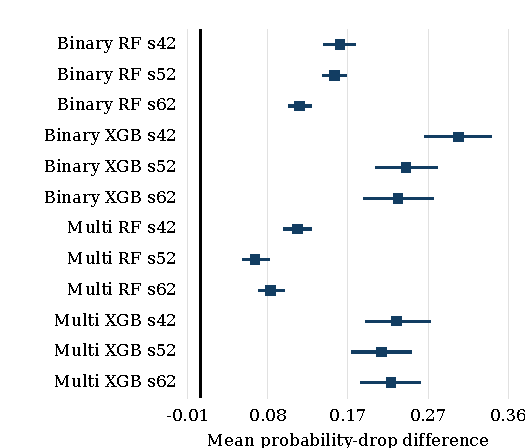
\includegraphics[width=\columnwidth]{figures/paired-1.pdf}
\caption{GeNIS paired connection-group mean differences with 95\% bootstrap intervals. Blue denotes Holm-adjusted directional p \ensuremath{<} 0.05; gray denotes non-significance. Each row is one model seed on the frozen split.}
\label{fig:1}
\end{figure}
\begin{figure}[!t]\centering
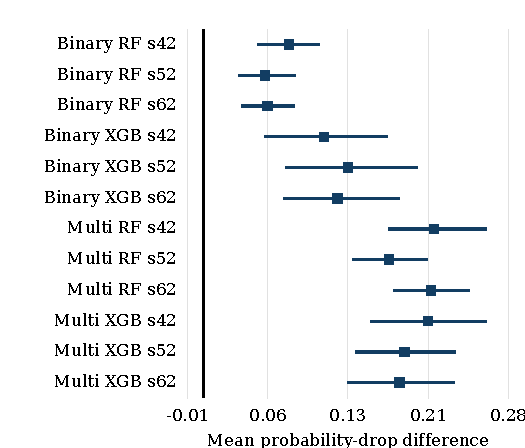
\includegraphics[width=\columnwidth]{figures/paired-2.pdf}
\caption{Gotham paired connection-group mean differences with 95\% bootstrap intervals. Blue denotes Holm-adjusted directional p \ensuremath{<} 0.05; gray denotes non-significance. Each row is one model seed on the frozen split.}
\label{fig:2}
\end{figure}
\begin{table}[!t]\centering
\caption{Paired differences across three model seeds}
\label{tab:5}
\footnotesize\setlength{\tabcolsep}{2pt}\renewcommand{\arraystretch}{1.10}
\begin{tabular}{>{\centering\arraybackslash}p{\dimexpr 0.17000\columnwidth-2\tabcolsep\relax}>{\centering\arraybackslash}p{\dimexpr 0.22000\columnwidth-2\tabcolsep\relax}>{\centering\arraybackslash}p{\dimexpr 0.18000\columnwidth-2\tabcolsep\relax}>{\centering\arraybackslash}p{\dimexpr 0.29000\columnwidth-2\tabcolsep\relax}>{\centering\arraybackslash}p{\dimexpr 0.14000\columnwidth-2\tabcolsep\relax}}\toprule
\textbf{Dataset} & \textbf{Task / model} & \textbf{Groups range} & \textbf{Mean delta range} & \textbf{Sig. / 3} \\\midrule
GeNIS & Binary RF & 93-93 & 0.117 to 0.165 & 3 / 3 \\
GeNIS & Binary XGB & 93-94 & 0.234 to 0.306 & 3 / 3 \\
GeNIS & Multi RF & 95-95 & 0.065 to 0.115 & 3 / 3 \\
GeNIS & Multi XGB & 95-95 & 0.215 to 0.232 & 3 / 3 \\
Gotham & Binary RF & 57-57 & 0.057 to 0.079 & 3 / 3 \\
Gotham & Binary XGB & 57-57 & 0.111 to 0.134 & 3 / 3 \\
Gotham & Multi RF & 63-63 & 0.172 to 0.213 & 3 / 3 \\
Gotham & Multi XGB & 63-63 & 0.182 to 0.208 & 3 / 3 \\
\bottomrule\end{tabular}\end{table}
\begin{table}[!t]\centering
\caption{Top-ranked masking relative to random control}
\label{tab:6}
\footnotesize\setlength{\tabcolsep}{2pt}\renewcommand{\arraystretch}{1.10}
\begin{tabular}{>{\centering\arraybackslash}p{\dimexpr 0.18000\columnwidth-2\tabcolsep\relax}>{\centering\arraybackslash}p{\dimexpr 0.21000\columnwidth-2\tabcolsep\relax}>{\centering\arraybackslash}p{\dimexpr 0.18000\columnwidth-2\tabcolsep\relax}>{\centering\arraybackslash}p{\dimexpr 0.18000\columnwidth-2\tabcolsep\relax}>{\centering\arraybackslash}p{\dimexpr 0.25000\columnwidth-2\tabcolsep\relax}}\toprule
\textbf{Dataset} & \textbf{Explainer} & \textbf{Positive lift / n} & \textbf{CI + Holm / n} & \textbf{Lift range} \\\midrule
GeNIS & LIME & 12/12 & 12/12 & 0.033 to 0.231 \\
GeNIS & TreeSHAP & 12/12 & 12/12 & 0.156 to 0.393 \\
Gotham & LIME & 12/12 & 8/12 & 0.015 to 0.307 \\
Gotham & TreeSHAP & 12/12 & 12/12 & 0.104 to 0.494 \\
\bottomrule\end{tabular}\end{table}
Table VI asks whether the ranking is informative under the same synthetic intervention. CI + Holm requires a positive lower 95\% group-bootstrap bound together with Holm-adjusted directional p \ensuremath{<} 0.05. Every top-minus-random hypothesis is adjusted in the 48-test family. 4 contexts (Gotham binary LIME) have positive mean lift and significant directional tests but intervals that cross zero, so they fail the combined criterion. Bottom-ranked scores remain in the artifacts as a descriptive check. An explainer comparison alone cannot show that either ranking improves over a random ranking.

\subsection{Latency, neighborhood similarity, and feature reduction}
\begin{table}[!t]\centering
\caption{Mean of three context medians and cosine means}
\label{tab:7}
\footnotesize\setlength{\tabcolsep}{2pt}\renewcommand{\arraystretch}{1.10}
\begin{tabular}{>{\centering\arraybackslash}p{\dimexpr 0.18000\columnwidth-2\tabcolsep\relax}>{\centering\arraybackslash}p{\dimexpr 0.23000\columnwidth-2\tabcolsep\relax}>{\centering\arraybackslash}p{\dimexpr 0.30000\columnwidth-2\tabcolsep\relax}>{\centering\arraybackslash}p{\dimexpr 0.29000\columnwidth-2\tabcolsep\relax}}\toprule
\textbf{Dataset} & \textbf{Task / model} & \textbf{SHAP / LIME ms} & \textbf{SHAP / LIME cosine} \\\midrule
GeNIS & Binary RF & 1.62 / 50.49 & 0.953 / 0.809 \\
GeNIS & Binary XGB & 0.99 / 26.16 & 0.956 / 0.870 \\
GeNIS & Multi RF & 2.59 / 66.68 & 0.970 / 0.683 \\
GeNIS & Multi XGB & 2.07 / 35.56 & 0.954 / 0.566 \\
Gotham & Binary RF & 2.93 / 42.04 & 0.992 / 0.922 \\
Gotham & Binary XGB & 1.15 / 8.80 & 0.981 / 0.860 \\
Gotham & Multi RF & 13.47 / 33.03 & 0.987 / 0.924 \\
Gotham & Multi XGB & 5.75 / 10.05 & 0.982 / 0.871 \\
\bottomrule\end{tabular}\end{table}
Table VII keeps each dataset/task/model context visible rather than combining correlated rows into one inferential claim. Timing excludes explainer construction and the complete IDS path, and background project-job contention was not controlled; the artifact additionally saves p90, p95, p99, throughput, top-5 overlap, and LIME repeatability. The reciprocal call-time throughput is not production IDS throughput. Neighborhood similarity depends on the chosen comparison set and representation, so it should not be called adversarial robustness.

\begin{table}[!t]\centering
\caption{Feature ablation; legacy label-union macro-f1}
\label{tab:8}
\footnotesize\setlength{\tabcolsep}{2pt}\renewcommand{\arraystretch}{1.10}
\begin{tabular}{>{\centering\arraybackslash}p{\dimexpr 0.16000\columnwidth-2\tabcolsep\relax}>{\centering\arraybackslash}p{\dimexpr 0.24000\columnwidth-2\tabcolsep\relax}>{\centering\arraybackslash}p{\dimexpr 0.15000\columnwidth-2\tabcolsep\relax}>{\centering\arraybackslash}p{\dimexpr 0.15000\columnwidth-2\tabcolsep\relax}>{\centering\arraybackslash}p{\dimexpr 0.15000\columnwidth-2\tabcolsep\relax}>{\centering\arraybackslash}p{\dimexpr 0.15000\columnwidth-2\tabcolsep\relax}}\toprule
\textbf{Dataset} & \textbf{Task / model} & \textbf{5 features} & \textbf{10 features} & \textbf{20 features} & \textbf{All} \\\midrule
GeNIS & Binary RF & 0.9998 & 0.9998 & 0.9998 & 0.9998 \\
GeNIS & Binary XGB & 0.9987 & 0.9998 & 0.9998 & 1.0000 \\
GeNIS & Multi RF & 0.9996 & 0.9996 & 0.9996 & 0.9997 \\
GeNIS & Multi XGB & 0.9888 & 0.9999 & 0.9999 & 1.0000 \\
Gotham & Binary RF & 0.9934 & 1.0000 & N/A & 1.0000 \\
Gotham & Binary XGB & 0.9946 & 0.9994 & N/A & 0.9999 \\
Gotham & Multi RF & 0.7630 & 0.8242 & N/A & 0.8238 \\
Gotham & Multi XGB & 0.4809 & 0.7661 & N/A & 0.8674 \\
\bottomrule\end{tabular}\end{table}
Feature reduction results are exploratory seed-42 refits and use the default true/predicted-label union macro-F1, which can include a predicted training-only class. They therefore use a different label averaging definition from Table II. N/A means the nominal subset exceeds the available predictor count. Requested counts are capped in the raw experiment, so repeated full-count rows are displayed once under All. The ranking is fitted on training data, but comparing multiple subsets on the held-out test set does not constitute independently validated feature selection. Any final subset should be fixed and confirmed on a new holdout. SHAP latency measured in this ablation is a small batched probe and is not directly interchangeable with Table VII's warmed single-record timings.

\subsection{Sensitivity and calibration audits}
Additional seed-42 audits evaluate binary calibration on the test cohort (Table IX), weighted versus unweighted fitting, TreeSHAP masking under five baselines on 12 diagnostic records, and LIME perturbation budgets 100, 350, and 700 on six records with five repeats (Table X). These small sensitivity cohorts provide descriptive checks; they are not independent confirmatory studies or a replacement for the paired group-level primary endpoint.

\begin{table}[!t]\centering
\caption{Binary seed-42 calibration on the capped cohort}
\label{tab:9}
\footnotesize\setlength{\tabcolsep}{2pt}\renewcommand{\arraystretch}{1.10}
\begin{tabular}{>{\centering\arraybackslash}p{\dimexpr 0.48000\columnwidth-2\tabcolsep\relax}>{\centering\arraybackslash}p{\dimexpr 0.26000\columnwidth-2\tabcolsep\relax}>{\centering\arraybackslash}p{\dimexpr 0.26000\columnwidth-2\tabcolsep\relax}}\toprule
\textbf{Dataset / model} & \textbf{Brier} & \textbf{10-bin ECE} \\\midrule
GeNIS RF & 0.0001 & 0.0010 \\
GeNIS XGB & 0.0002 & 0.0002 \\
Gotham RF & 0.0001 & 0.0026 \\
Gotham XGB & 0.0000 & 0.0002 \\
\bottomrule\end{tabular}\end{table}
Across the eight contexts, descriptive TreeSHAP mean deletion scores under the masking alternatives are marginal training row: 0.360; nearest opposite prediction: 0.539; nearest same prediction: -0.005; training median mode: 0.423; zero: 0.290. This pooling is a sensitivity summary only. Baseline-dependent scores reinforce that the masking intervention is part of the measured construct.

\begin{table}[!t]\centering
\caption{Descriptive lime budget audit, contexts pooled}
\label{tab:10}
\footnotesize\setlength{\tabcolsep}{2pt}\renewcommand{\arraystretch}{1.10}
\begin{tabular}{>{\centering\arraybackslash}p{\dimexpr 0.24000\columnwidth-2\tabcolsep\relax}>{\centering\arraybackslash}p{\dimexpr 0.25000\columnwidth-2\tabcolsep\relax}>{\centering\arraybackslash}p{\dimexpr 0.25000\columnwidth-2\tabcolsep\relax}>{\centering\arraybackslash}p{\dimexpr 0.26000\columnwidth-2\tabcolsep\relax}}\toprule
\textbf{LIME samples} & \textbf{Deletion} & \textbf{Repeat cosine} & \textbf{Median ms} \\\midrule
100 & 0.222 & 0.702 & 26.70 \\
350 & 0.232 & 0.834 & 29.84 \\
700 & 0.252 & 0.872 & 33.56 \\
\bottomrule\end{tabular}\end{table}
Class-weighted minus unweighted test-supported-label macro-F1 varies from -0.0043 to 0.0000 across seed-42 contexts. Calibration values apply to the known-label capped test cohort; they do not estimate calibration at natural deployment prevalence. The LIME budget audit reuses seeds and records and is presented without a pooled significance claim.

\section{Discussion and threats to validity}
The refreshed evidence addresses the missing local conversion history by making the source-to-cohort transformation inspectable and rerunnable. It does not retrospectively recover the legacy parquet provenance. Source snapshots and hashes fix the consumed author files and executed transformations, while the narrower Gotham member-verification scope remains a declared limitation. CRC32 detects transfer or extraction inconsistency; it is not a publisher-signed cryptographic authenticity proof.

The group split prevents the chosen connection keys from crossing partitions. It is not a device-disjoint, scenario-disjoint, forward-in-time, cross-network, or external-attack evaluation. GeNIS scenarios can share testbed material beyond FlowID, and Gotham endpoint tuples can merge repeated sessions or leave other correlations across different tuples. Equal feature patterns across groups remain in the primary cohort. High performance can therefore coexist with limited external validity.

The class cap changes prevalence and can underrepresent rare attack diversity. Unknown-labelled packets are outside both supervised tasks. A label confined to one group cannot support an independent test claim; the supported-class macro-F1 is restricted to labels present in test. Five predictive seeds share one preparation seed and one split; they do not explore split uncertainty. Explanation sampling prioritizes error types, and the inferential population is the explained groups represented by this selection rather than every packet in the full dataset. Group means reduce within-key dependence but do not remove all dependence across groups or model seeds.

The directional TreeSHAP-greater test permits checking that specific hypothesis; a reverse claim requires a separately specified analysis. Bootstrap intervals are per context and are not simultaneous confidence intervals, whereas Holm controls the reported hypothesis families. The default TreeSHAP value function and LIME's discretized local surrogate can respond differently to correlated and categorical predictors. Masking by a mixed median/mode vector can create off-manifold combinations, so a larger deletion drop is a protocol-specific ranking result.

This work has no participant study, production monitoring, packet-capture throughput benchmark, drift test, or attack intervention study. Gaspar \emph{et al.} \cite{ref14} include a perceived-interpretability survey; our work has no corresponding human evidence. Neither our deletion results nor that survey establish operational alert cost, current attack coverage, or adversarial safety. A stronger next evaluation would freeze the chosen configuration, use a separately captured device/scenario/time holdout, retain natural prevalence for operational calibration, and measure analyst decisions with a pre-specified human study.

\section{Reproducibility and reporting status}
The executed environment uses Python 3.12.14, scikit-learn 1.6.1, XGBoost 3.0.2, SHAP 0.47.2, and LIME 0.2.0.1. The project saves author-record metadata, acquisition and per-member hashes, exclusions, source row counts, class counts, split and overlap audits, prepared parquet hashes, source snapshots, fitted seed-42 models, and per-context checkpoints. The configuration and source hashes in run\_manifest.json define this run. Artifact verification checks coverage and internal consistency; it is not independent external replication.

A clean rerun begins with the official acquisition scripts, then deterministic preparation, the recent-data benchmark, and artifact verification. It requires the author data downloads and the pinned requirements. The benchmark caps are part of the experiment and should not be silently replaced with full-data or per-file caps. No repository release, archival DOI, or externally executed replication is claimed in this draft.

\textbf{AI assistance disclosure:} OpenAI Codex assisted with source acquisition tooling, data auditing, experiment orchestration, and manuscript drafting. The authors must verify the methods, results, citations, and disclosure against the selected venue's requirements and accept responsibility for the final work. No specific IEEE journal or conference has been selected. The generic IEEE conference format used here does not establish compliance with a selected venue's submission requirements.

\section{Conclusion}
Two official author releases from 2025 now supply traceable primary inputs for the intrusion-detection explanation benchmark. The frozen group-aware protocol produces 40 predictive fits, 24 paired explainer contexts, and 48 random-control tests. TreeSHAP has a positive mean deletion difference in 24/24 contexts and meets the directional Holm-adjusted criterion in 24/24. The contribution is this provenance-traceable, group-aware evaluation protocol rather than a new explainer. These findings are limited to the sampled cohorts, explanation budgets, masks, and connection-group holdout. Dataset provenance is documented for the new cohorts; legacy conversion provenance remains unresolved and its results remain historical.

\begin{thebibliography}{20}
\bibitem{ref1} M. Silva, D. Pinto, J. Vitorino, J. Gonçalves, E. Maia, and I. Praça, "GeNIS: GECAD Network Intrusion Scenarios," Zenodo, ver. 1.0.0, Feb. 24, 2025, doi: \href{https://doi.org/10.5281/zenodo.14919237}{10.5281/zenodo.14919237}.
\bibitem{ref2} M. Silva, D. Pinto, J. Vitorino, J. Gonçalves, E. Maia, and I. Praça, "GeNIS: A modular dataset for network intrusion detection and classification," \emph{Data in Brief}, vol. 60, art. no. 111487, Jun. 2025, doi: \href{https://doi.org/10.1016/j.dib.2025.111487}{10.1016/j.dib.2025.111487}.
\bibitem{ref3} O. Belarbi, T. Spyridopoulos, E. Anthi, O. Rana, P. Carnelli, and A. Khan, "A Device-Level IoT Network Traffic Dataset with Distributed Capture and Non-IID Characteristics," Zenodo, ver. v1, Feb. 5, 2025, doi: \href{https://doi.org/10.5281/zenodo.14502760}{10.5281/zenodo.14502760}.
\bibitem{ref4} O. Belarbi, T. Spyridopoulos, E. Anthi, O. Rana, P. Carnelli, and A. Khan, "Gotham Dataset 2025: A Reproducible Large-Scale IoT Network Dataset for Intrusion Detection and Security Research," arXiv:2502.03134, ver. 1, Feb. 5, 2025, doi: \href{https://doi.org/10.48550/arXiv.2502.03134}{10.48550/arXiv.2502.03134}.
\bibitem{ref5} L. Breiman, "Random forests," \emph{Machine Learning}, vol. 45, no. 1, pp. 5-32, 2001, doi: \href{https://doi.org/10.1023/A:1010933404324}{10.1023/A:1010933404324}.
\bibitem{ref6} T. Chen and C. Guestrin, "XGBoost: A scalable tree boosting system," in \emph{Proc. ACM SIGKDD}, 2016, pp. 785-794, doi: \href{https://doi.org/10.1145/2939672.2939785}{10.1145/2939672.2939785}.
\bibitem{ref7} S. M. Lundberg and S.-I. Lee, "A unified approach to interpreting model predictions," in \emph{Advances in Neural Information Processing Systems}, vol. 30, 2017. [Online]. Available: \href{https://proceedings.neurips.cc/paper/2017/hash/8a20a8621978632d76c43dfd28b67767-Abstract.html}{NeurIPS proceedings}.
\bibitem{ref8} S. M. Lundberg \emph{et al.}, "From local explanations to global understanding with explainable AI for trees," \emph{Nature Machine Intelligence}, vol. 2, pp. 56-67, 2020, doi: \href{https://doi.org/10.1038/s42256-019-0138-9}{10.1038/s42256-019-0138-9}.
\bibitem{ref9} M. T. Ribeiro, S. Singh, and C. Guestrin, "Why should I trust you?": Explaining the predictions of any classifier, in \emph{Proc. ACM SIGKDD}, 2016, pp. 1135-1144, doi: \href{https://doi.org/10.1145/2939672.2939778}{10.1145/2939672.2939778}.
\bibitem{ref10} C.-K. Yeh, C.-Y. Hsieh, A. S. Suggala, D. I. Inouye, and P. Ravikumar, "On the (in)fidelity and sensitivity of explanations," in \emph{Advances in Neural Information Processing Systems}, vol. 32, 2019. [Online]. Available: \href{https://proceedings.neurips.cc/paper/2019/hash/a7471fdc77b3435276507cc8f2dc2569-Abstract.html}{NeurIPS proceedings}.
\bibitem{ref11} J. Adebayo, J. Gilmer, M. Muelly, I. Goodfellow, M. Hardt, and B. Kim, "Sanity checks for saliency maps," in \emph{Advances in Neural Information Processing Systems}, vol. 31, 2018. [Online]. Available: \href{https://proceedings.neurips.cc/paper/2018/hash/294a8ed24b1ad22ec2e7efea049b8737-Abstract.html}{NeurIPS proceedings}.
\bibitem{ref12} S. Neupane \emph{et al.}, "Explainable intrusion detection systems (X-IDS): A survey of current methods, challenges, and opportunities," \emph{IEEE Access}, vol. 10, pp. 112392-112415, 2022, doi: \href{https://doi.org/10.1109/ACCESS.2022.3216617}{10.1109/ACCESS.2022.3216617}.
\bibitem{ref13} S. Mane and D. Rao, "Explaining network intrusion detection system using explainable AI framework," arXiv:2103.07110, ver. 1, Mar. 12, 2021, doi: \href{https://doi.org/10.48550/arXiv.2103.07110}{10.48550/arXiv.2103.07110}.
\bibitem{ref14} D. Gaspar, P. Silva, and C. Silva, "Explainable AI for intrusion detection systems: LIME and SHAP applicability on multi-layer perceptron," \emph{IEEE Access}, vol. 12, pp. 30164-30175, 2024, doi: \href{https://doi.org/10.1109/ACCESS.2024.3368377}{10.1109/ACCESS.2024.3368377}.
\bibitem{ref15} A. Warnecke, D. Arp, C. Wressnegger, and K. Rieck, "Evaluating explanation methods for deep learning in security," in \emph{Proc. IEEE Eur. Symp. Security and Privacy (EuroS\&P)}, 2020, pp. 158-174, doi: \href{https://doi.org/10.1109/EuroSP48549.2020.00018}{10.1109/EuroSP48549.2020.00018}.
\bibitem{ref16} O. Arreche, T. R. Guntur, J. W. Roberts, and M. Abdallah, "E-XAI: Evaluating black-box explainable AI frameworks for network intrusion detection," \emph{IEEE Access}, vol. 12, pp. 23954-23988, 2024, doi: \href{https://doi.org/10.1109/ACCESS.2024.3365140}{10.1109/ACCESS.2024.3365140}.
\bibitem{ref17} I. C. Covert, S. Lundberg, and S.-I. Lee, "Explaining by removing: A unified framework for model explanation," \emph{Journal of Machine Learning Research}, vol. 22, no. 209, pp. 1-90, 2021. [Online]. Available: \href{https://jmlr.org/papers/v22/20-1316.html}{JMLR 20-1316}.
\bibitem{ref18} B. Efron, "Bootstrap methods: Another look at the jackknife," \emph{Annals of Statistics}, vol. 7, no. 1, pp. 1-26, 1979, doi: \href{https://doi.org/10.1214/aos/1176344552}{10.1214/aos/1176344552}.
\bibitem{ref19} F. Wilcoxon, "Individual comparisons by ranking methods," \emph{Biometrics Bulletin}, vol. 1, no. 6, pp. 80-83, 1945. [Online]. Available: \href{https://www.jstor.org/stable/3001968}{JSTOR 3001968}.
\bibitem{ref20} S. Holm, "A simple sequentially rejective multiple test procedure," \emph{Scandinavian Journal of Statistics}, vol. 6, no. 2, pp. 65-70, 1979. [Online]. Available: \href{https://www.jstor.org/stable/4615733}{JSTOR 4615733}.
\end{thebibliography}
\end{document}